In order to test the effectiveness of IISVMs with respect to standard
SVMs, we have chosen two standard benchmarks for machine learning
methods, namely the the \emph{Haberman} and the \emph{Diabetes}
suites, and have then run comparative tests on them. In order to check
our predictions about the linear independence tolerance constant,
$\eta$, we have chosen finite- and infinite-dimensional kernels,
namely polynomial kernels of degree $1$ (linear) and cubic, and
Gaussian kernel. We expect, in the finite-dimensional case, $\eta$ to
be essentially irrelevant, and the machine to stop growing once a
certain number of l.i. support vectors have been found. This is
exactly due to the feature space being finite-dimensional, and
therefore only a finite number of l.i. vectors can be found. In the
case of the infinite-dimensional kernel, we have run the IISVM with
$\eta$ at different values, expecting, as foretold, bigger values of
$\eta$ to cause the accuracy to degrade, but also the size of the
machine to remain smaller than with smaller values.

We have implemented IISVMs in Matlab, using the code made available by
Keerthi et al. \cite{KeerthiCDC06}. Since this is a fast prototyping
implementation, CPU times are not relevant to the discussion. As an
aside note, IISVMs are so far slower than Keerthi et al.'s machines,
but it must be remembered that their approach is approximate, while
ours, if $\eta$ is set to machine precision, is not approximate.

Figures \ref{fig:finite} and \ref{fig:infinite} show the results. For
each benchmark, we display the mean number of retained support vectors
on $5$ random $75\%/25\%$ train/test runs (y-axis), as more training
samples are acquired (x-axis). We compare against LIBSVM
\cite{ChangL01} (straight line), a standard SVM implementation. (The
coefficients $\gamma$ and $C$ have been found by cross-validation and
employed in both LIBSVM and IISVMs. For the sake of comparison, LIBSVM
has been modified as suggested by the Authors in order to use the
squared norm of $\ww$ in the cost function. Therefore in the following
it is called LIBSVM-2.) In the case of finite-dimensional kernels, we
only show the performance of LIBSVM-2 against IISVMs with $\eta$ at
machine precision; in the case of the infinite-dimensional kernel, we
show curves for various values of $\eta$.

%% \begin{figure*}[!htbp]
%%   \begin{center}
%%     \begin{tabular}{cc}
%%        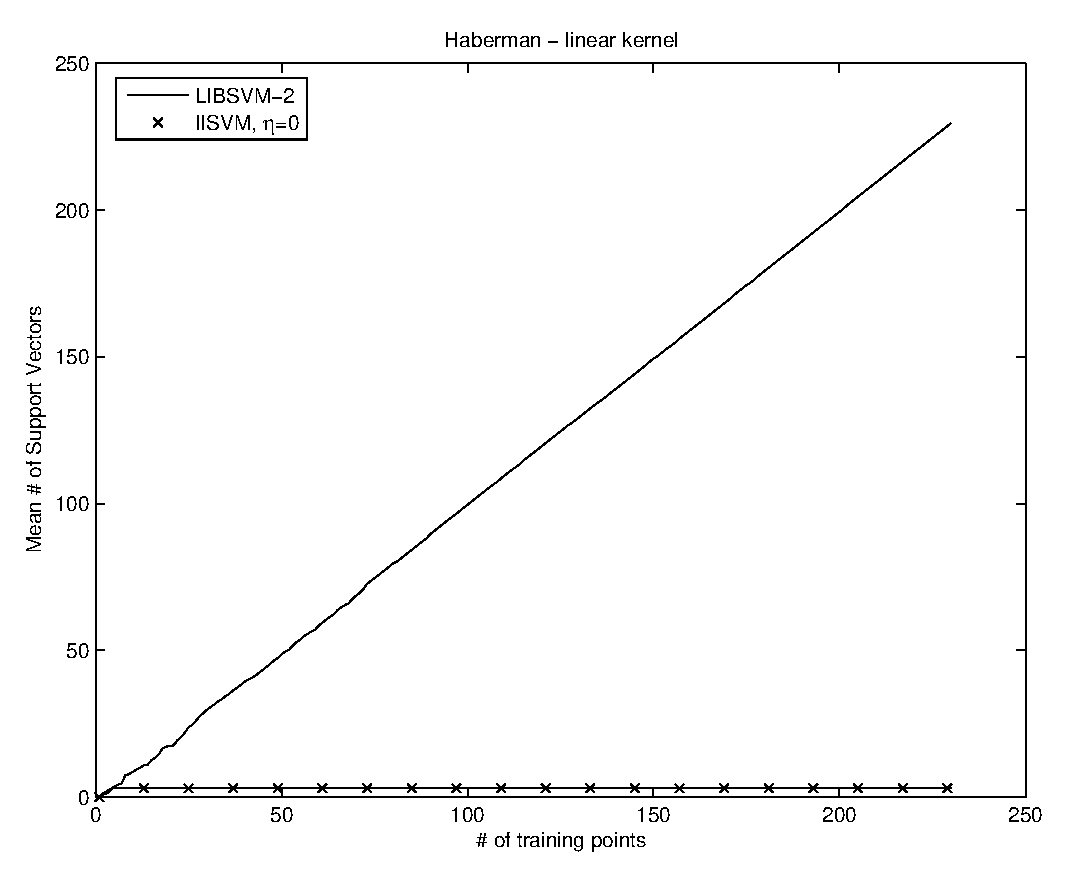
\includegraphics[width=0.45\textwidth]{Haberman_lin} &
%%        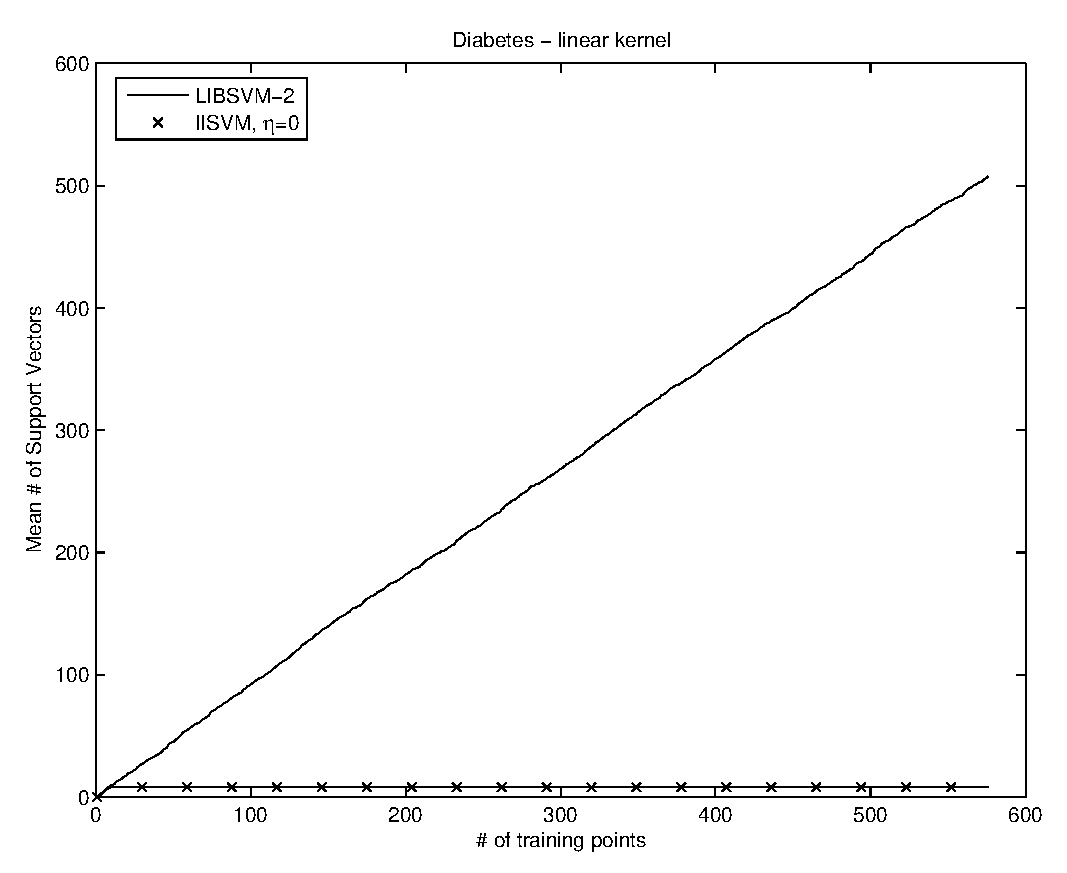
\includegraphics[width=0.45\textwidth]{Diabetes_lin} \\
%%        \multicolumn{2}{c}{(a)} \\
%%        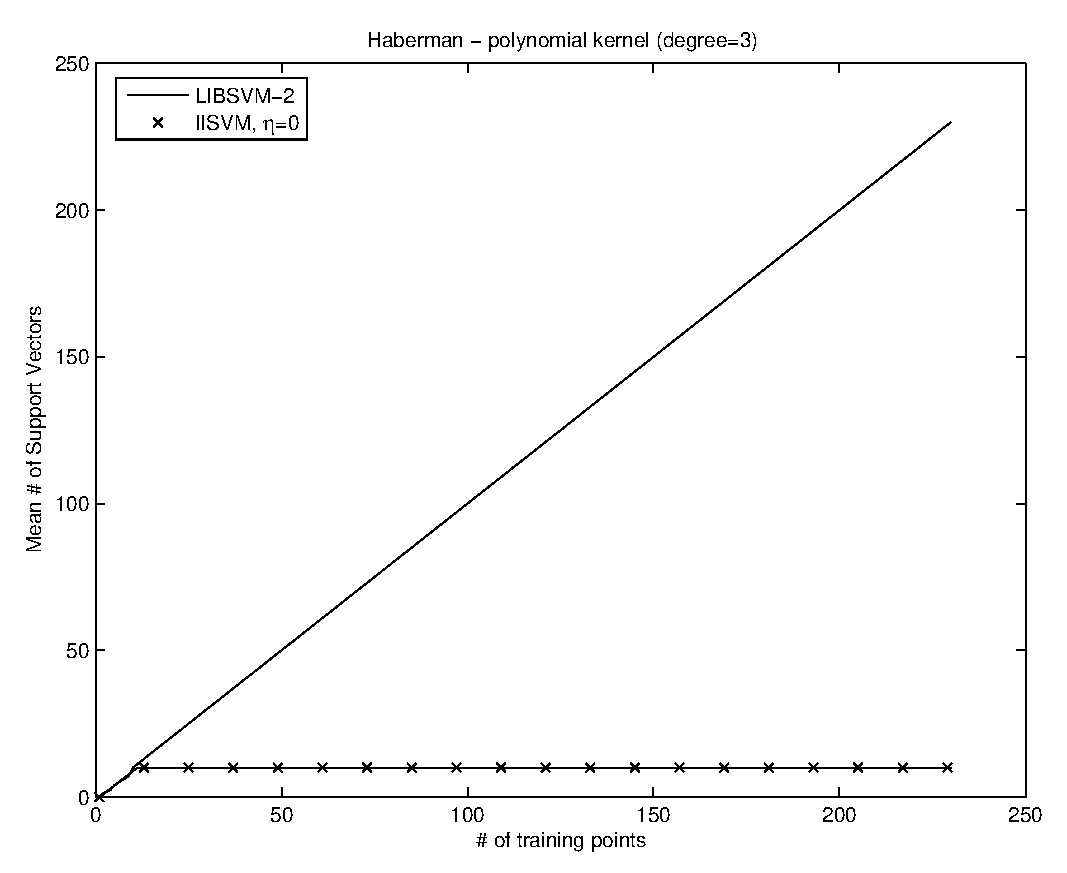
\includegraphics[width=0.45\textwidth]{Haberman_poly3} &
%%        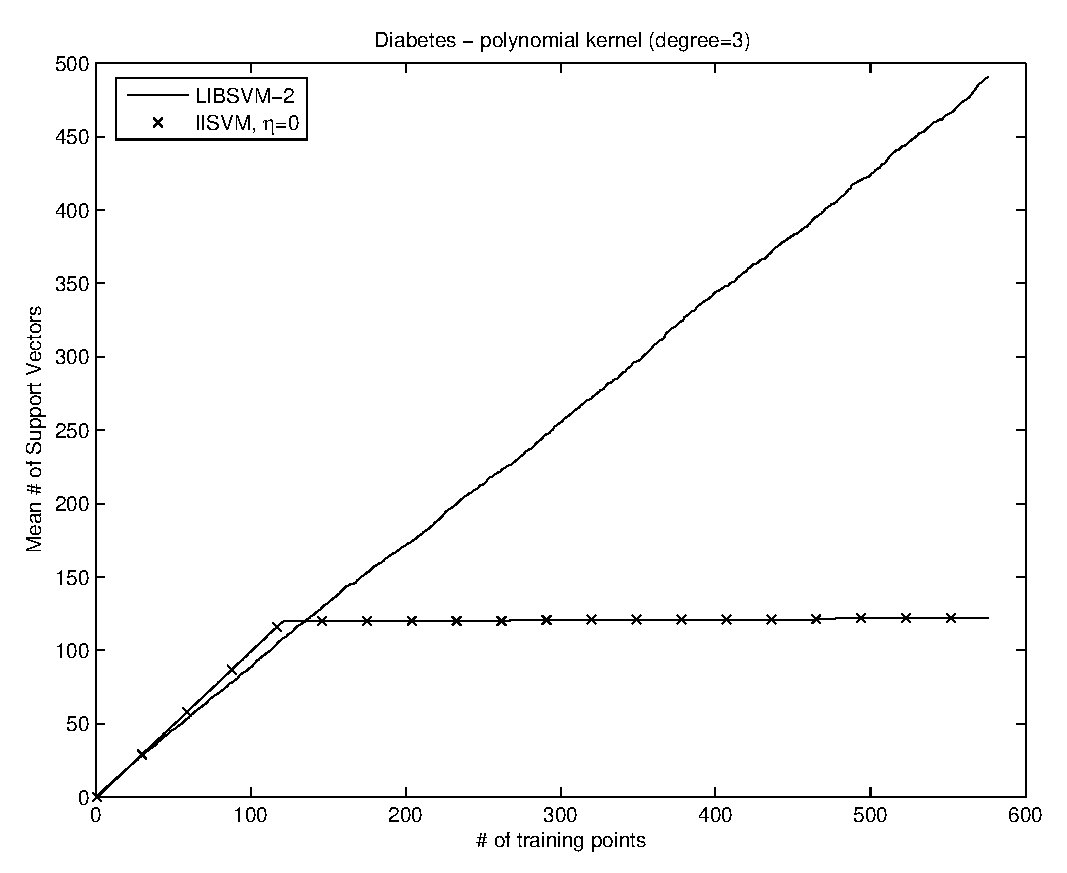
\includegraphics[width=0.45\textwidth]{Diabetes_poly3} \\
%%        \multicolumn{2}{c}{(b)} \\
%%     \end{tabular}
%%   \end{center}
%%   \caption{\label{fig:finite} test results with finite-dimensional
%%   kernels: (a) linear kernel, (b) polynomial kernel with degree $3$.}
%% \end{figure*}

%% \begin{figure*}[!htbp]
%%   \begin{center}
%%     \begin{tabular}{cc}
%%        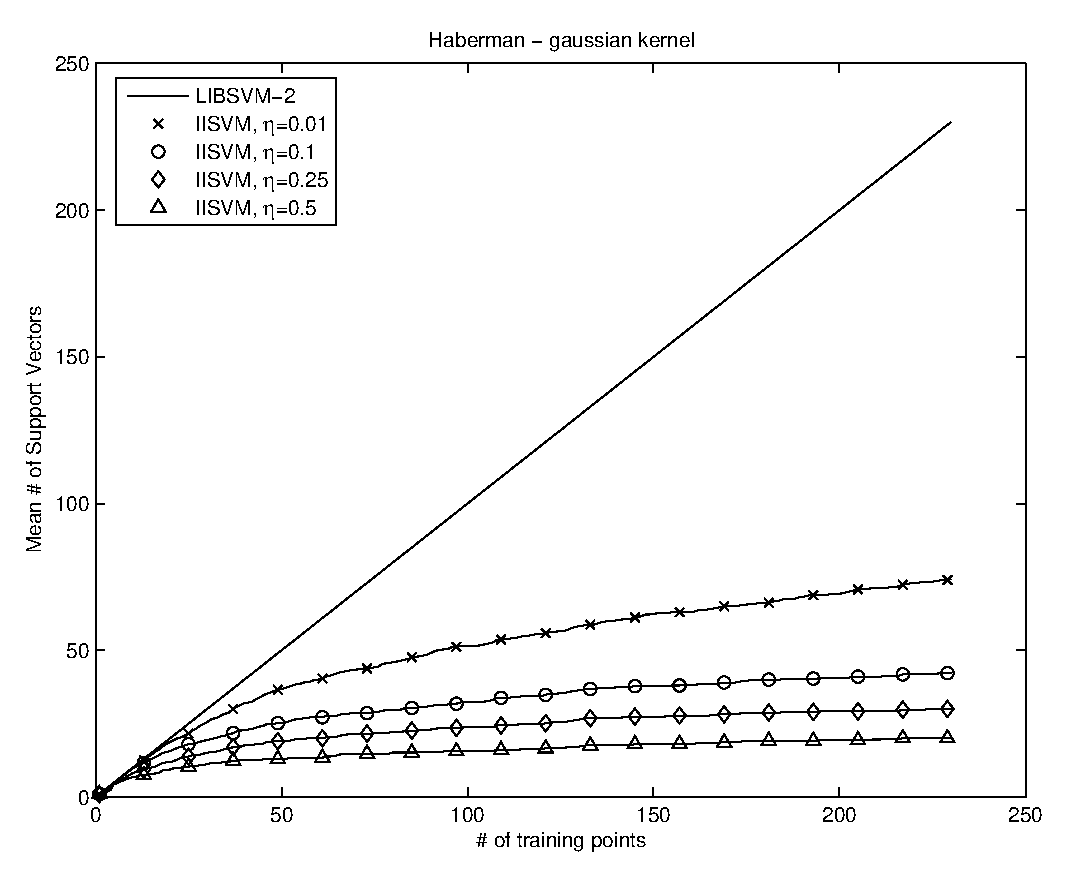
\includegraphics[width=0.45\textwidth]{Haberman_gaussian} &
%%        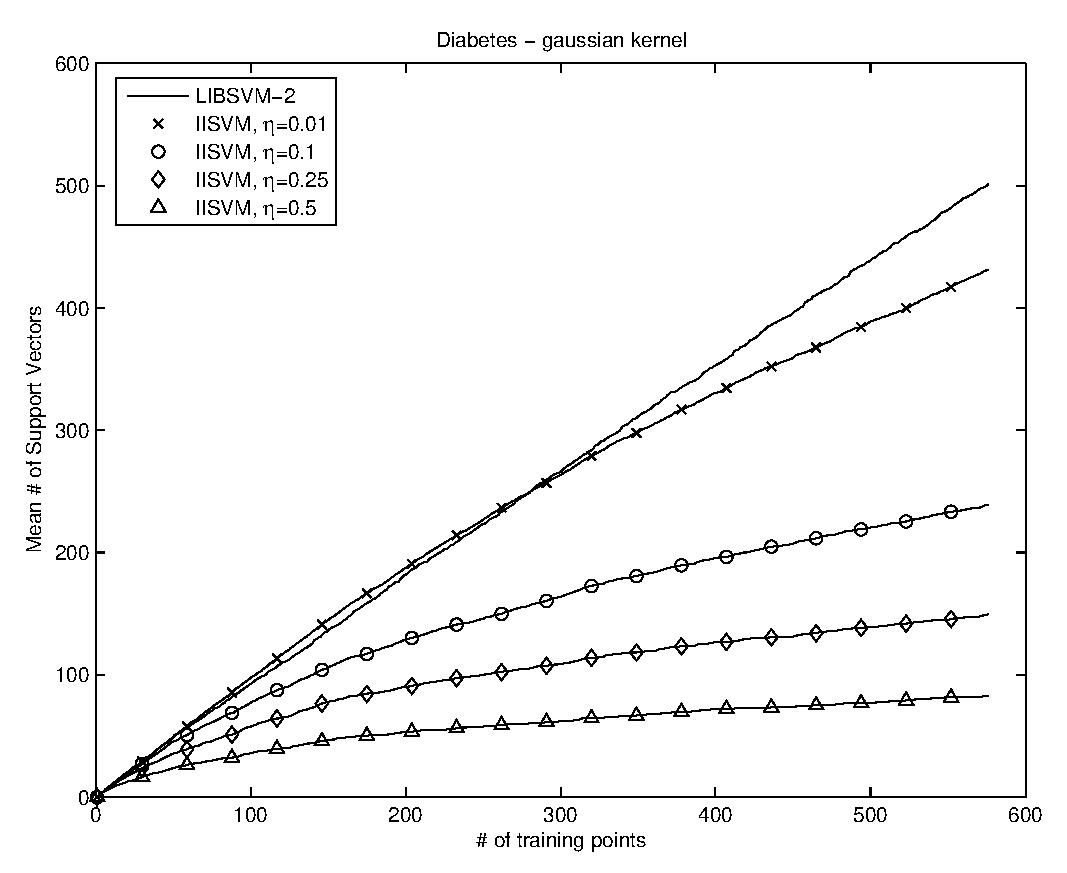
\includegraphics[width=0.45\textwidth]{Diabetes_gaussian}
%%     \end{tabular}
%%   \end{center}
%%   \caption{\label{fig:infinite} test results with an infinite-dimensional
%%   (Gaussian) kernel.}
%% \end{figure*}

Consider Figure \ref{fig:finite}: as one can see, as opposed to the
linear behaviour of LIBSVM-2, IISVMs quickly attain a constant number
of support vectors and then stop acquiring new ones. The values are,
in turn, $3$ support vectors in Figure \ref{fig:finite}(a) and $10$
and $120$ in Figure \ref{fig:finite}(b). These numbers match exactly
the dimensions of the related feature spaces, given by
$\binom{m+deg-1}{deg}$ where $deg$ is the degree of the polynomial
kernel (obviously $1$ in the case of linear kernels).

Consider Figure \ref{fig:infinite}: in this case IISVMs obtains a
dramatic reduction in the number of support vectors, as expected, as
the tolerance threshold $\eta$ is made larger and larger. Also, the
shape of the curve seems in most cases to be no longer linear but
rather somehow logarithmic. As $\eta$ is raised, as expected, the
relative error\footnote{let $e$ and $e'$ be the error obtained
in turn by IISVM and LIBSVM-2; then the relative error is defined as
$(e'-e)/e'$.} with respect to LIBSVM-2 grows, but
in a remarkably small way: in the worst cases, that is for $\eta=0.5$,
the relative error is slightly more than $1\%$ with respect to
LIBSVM-2, whereas it is $0.24\%$ for the Haberman suite.

As a final remark, notice that in general the number of support
vectors chosen by IISVMs could be higher than that obtained by
SVMs. An example of this phenomenon is visible in Figure
\ref{fig:infinite}, right plot, between x-values $100$ and $200$.
